\documentclass[a4paper]{article}
\usepackage{amsmath}
\usepackage{amsfonts}
\usepackage{amsthm}
\usepackage{amssymb}
\usepackage[english]{babel}
\usepackage{float}
\usepackage{graphicx}
\usepackage{hyperref}
\usepackage[utf8]{inputenc}
\usepackage{listings}
\usepackage{xcolor}
%% \usepackage{subfigure}
\usepackage{graphicx}
\usepackage{subcaption}
\usepackage{stmaryrd}

\usepackage{a4wide}
\usepackage{url}

\usepackage{appendix}

\graphicspath{{imgs/}} %Setting the graphicspath

\lstset{
  frame=tb,
  language=Python,
  aboveskip=3mm,
  belowskip=3mm,
  showstringspaces=false,
  formfeed=newpage,
  tabsize=4,
  comment=[l]{\#},
  breaklines=true,
  morekeywords={models, lambda, forms}
}

\newcommand{\prob}[1]{\mathbb{P}\left(#1\right)}
\newcommand{\expect}[1]{\mathbb{E}\left(#1\right)}
\newcommand{\bt}[1]{\mathbf{#1}}
\newcommand{\avg}[1]{\sum_{i=1}^{#1}X_i}
\newcommand*{\QEDA}{\hfill\ensuremath{\blacksquare}}%

\newcommand{\nt}{\text}
\newcommand{\lagr}{\mathcal{L}}
\newcommand{\isum}{\sum^\infty_}
\newcommand{\f}{$f$}

\title{\vspace{-5cm} Numerical Optimization \\ Re-exam Handin 5}
\author{Dmitry Serykh (qwl888)}

\begin{document}
\maketitle
\section{The Setup}
In this assignment, I have implemented the Trust Region algorithm, using
quasi-newton method with SR1 update as presented in Algorithm 6.2 in the book.

\subsection{Parameters}
I used following parameter values in my implementation. Some values were taken
from the literature, while others were determined empirically.
\begin{itemize}
\item I used an identity matrix for the $B_0$, since I could not find any
  information about the initial value of $B$ for the SR1 update in the book and
  none of my ad-hoc experiments led to any noticeable improvement.
\item \textbf{Initial trust region radius ($\Delta_0 = 1$)}
\item \textbf{Lower bound for the actual/predicted reduction ratio $\eta=0.01$}
\item \textbf{Tolerance $\varepsilon = 10^{-7}$ on the gradient magnitude}
\item \textbf{Lower bound on the update denominator $r=10^{-8}$}
\end{itemize}

\section{Testing protocol}
In order to test the effectiveness of my implementation, I came up with a
testing protocol, where I used following metrics:
\begin{itemize}
\item The convergence plots with the number of iteration on the x-scale and the
  Euclidean distance between the current value of $x$ and the
  optimum. The resulting plot can be seen on Figure \ref{plt1}.
\item The convergence plots with gradient magnitude.
  The resulting plot can be seen on Figure \ref{plt2}. 
\item \textbf{Accuracy}. The Euclidean distance to the optimum at the
  termination point. The results can be seen on Table \ref{table1}.
  The performance of my implementation of the trust
  region algorithm is compared to the performance of the line search and trust
  region methods from Assignment 3 and 4.
\item \textbf{Efficiency}. The number of steps until the gradient
  magnitude reaches $10^{-7}$. The results can be seen on Table \ref{table2}.
\end{itemize}
I used a random starting point taken from the uniform distribution in the
interval between $-10$ to $10$ and repeated each optimization 100 times for all
metrics and took the median.


\begin{figure}[]
    \centering
    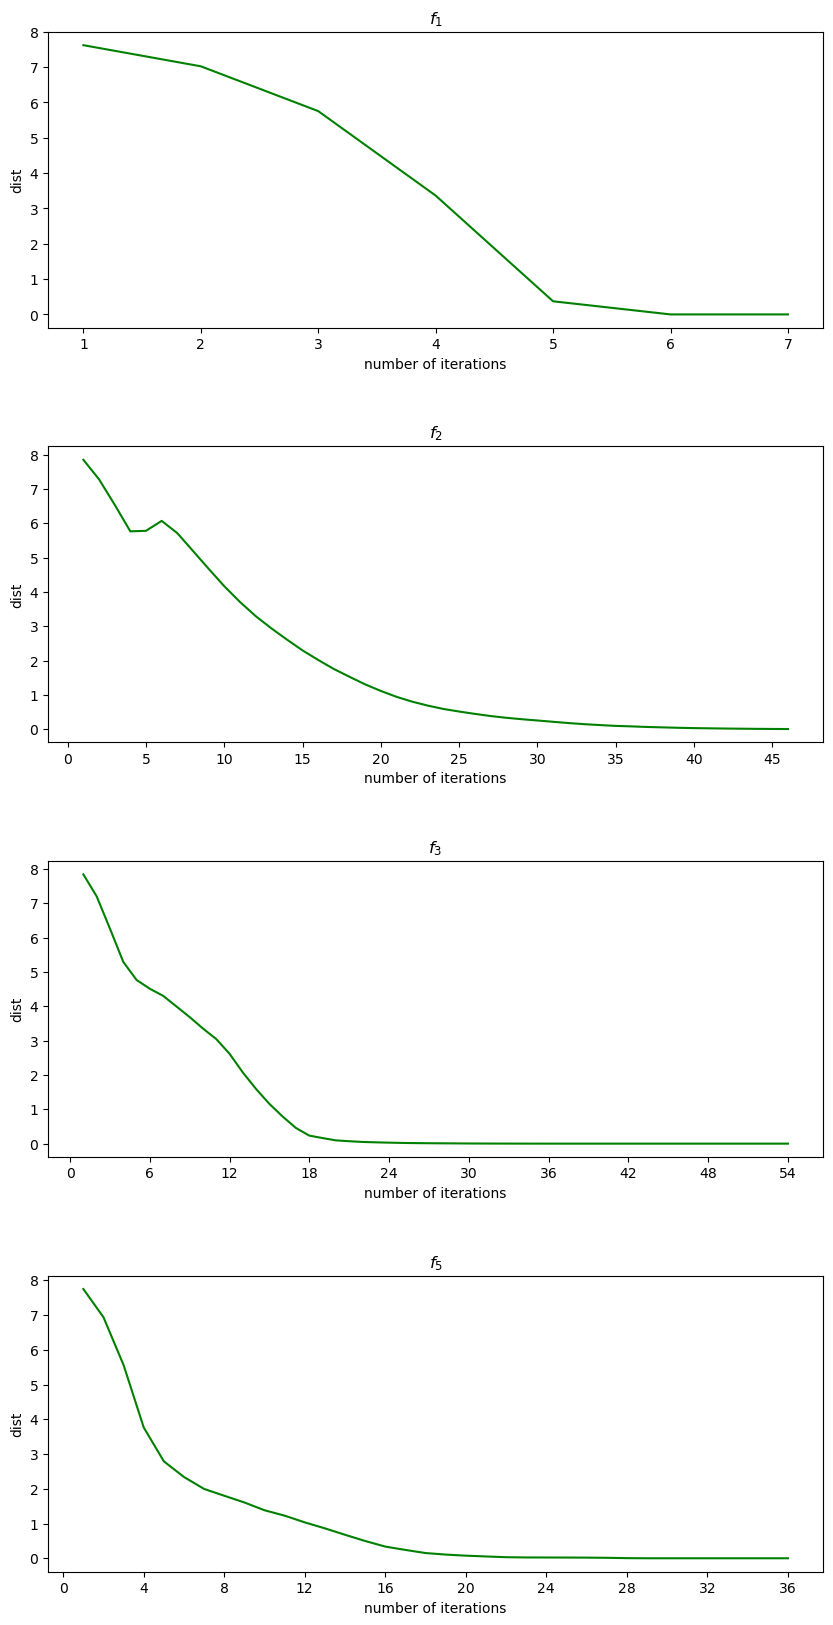
\includegraphics[width=0.7\textwidth]{plt_dist100.png}
    \caption{Convergence plot with euclidean distance to the optimum on the y-axis(log scale)}
  \label{plt1}
\end{figure}

\begin{figure}[]
    \centering
    \includegraphics[width=0.7\textwidth]{plt_grad_norm100.png}
    \caption{Plot of the gradient magnitude as a function of number of
      iterations (log scale)}
  \label{plt2}
\end{figure}

\begin{table}[]
\centering
\begin{tabular}{|l|l|l|l|l|l|}
\hline
                 & $f_1$         & $f_2$         & $f_3$       & $f_4$       & $f_5$       \\ \hline
stepest descent & $1.44\cdot10^{-4}$ & $7.59\cdot10^{-4}$ & $1.44\cdot10^{-10}$ & $6.51\cdot10^{-7}$ & $1.13\cdot 10^{-4}$ \\ \hline
newton           & $0.0$      & $8.15\cdot10^{-8}$ & $4.59\cdot10^{-16}$ & $6.4\cdot10^{-7}$  & $4.56\cdot10^{-7}$ \\ \hline
trust region    & $6.11\cdot 10^{-18}$  & $3.17\cdot 10^{-15}$ &  $1.08\cdot10^{-12}$ & n/a & $1.70 \cdot 10^{-7}$ \\ \hline
SR1 trust region  & $7.44 \cdot 10^{-17}$  & $7.38 \cdot 10^{-12}$ &  $2.40\cdot 10^{-12}$ & n/a & $2.71 \cdot 10^{-7}$ \\ \hline
\end{tabular}
\caption{Average value of distance to the optimum at algorithm termination for 100 random starting points in the interval $[-10,10]$}
\label{table1}
\end{table}

\begin{table}[]
\centering
\begin{tabular}{|l|l|l|l|l|l|}
\hline
                 & $f_1$  & $f_2$  & $f_3$   & $f_4$ & $f_5$  \\ \hline
stepest descent  & $3392$ & $6991$ & $5546$ & $488$ & $52$  \\ \hline
newton           & $1$    & $30$   & $16$   & $29$  & $2 $  \\ \hline
trust region     & $5$    & $32$   & $35$   & n/a   & $24 $ \\ \hline
SR1 trust region & $6$    & $73$   & $64$   & n/a   & $25 $ \\ \hline
\end{tabular}
\caption{Average number of iterations until algorithm termination for 100 random starting points in the interval $[-10,10]$}
\label{table2}
\end{table}

\section{Theoretical Part}
In the theoretical part, I will show that Newtons
Method is invariant to all invertible linear transformations of the objective
function.\\\\
Assume that Newtons Method with backtracking line-search is run on $f$ with starting point
$x_0$, producing a sequence of iterates $x_1, \dots x_T$
with step-candidates $p_1, \dots p_T$. Further, assume we
ran the algorithm on: $g(x)=f(Ax)$, where $A$ is
square and invertible and choose as starting-point $\tilde{x}_0= A^{-1}$
leading to iterates $\tilde{x}_1, \dots \tilde{x}_T$ with step candidates
$\tilde{p}_1, \dots \tilde{p}_T$.

\subsection{Step 1}
I will show that the hessian is $\nabla^2 g(x)= A^T \left[\nabla^2 f(Ax)\right] A$. This can be shown
by application of the chain rule. Hence, we get:
\begin{align*}
 g(x) &= f(Ax)\\
 \nabla g(x) &= A^T \nabla f(Ax)\\
 \nabla^2 g(x) &= A^T \left[\nabla^2 f(Ax)\right]A
\end{align*}

\subsection{Step 2}
Then, I assume that $\tilde{x}_k= A^{-1} x_k$ and show that
$\tilde{p}_k=A^{-1}p_k$. The search direction for the Newton's method is:
$-\nabla^{2}f^{-1}\nabla f$, therefore:
\[
\begin{aligned}
  \tilde{p}_{k} &=-(\nabla^{2} g\left(\tilde{x}_{k}\right)^{-1}) \nabla g\left(\tilde{x}_{k}\right) \\
  &=\left(-A^T \nabla^{2} f\left(x_{k}\right) A\right)^{-1} A^T \nabla f\left(x_{k}\right) \\
  &=-A^{-1} \nabla^{2} f\left(x_{k}\right)^{-1} (A^T)^{-1} A^T \nabla f\left(x_{k}\right) \\
  &=A^{-1}(- \nabla^{2} f\left(x_{k}\right)^{-1}) I \nabla f\left(x_{k}\right) \\
  &=A^{-1}\left(-\nabla^{2} f\left(x_{k}\right)^{-1} \nabla f\left(x_{k}\right)\right) \\
  &=A^{-1} p_{k}
\end{aligned}
\]

\subsection{Step 3}
Next, I will show that $\alpha_k$ stays the same after transformation.
We assumed that $\tilde{x} =  A^{-1}x$ and showed that $\tilde{p}_k=A^{-1}p_k$.
Therefore, we have:
\[
\begin{aligned}
  g(\tilde{x}_k+\alpha \tilde{p}_k)
  &= f(A(\tilde{x}_k+\alpha \tilde{p}_k))\\
  &= f(A\tilde{x}_k + A\alpha \tilde{p}_k)\\
  &= f(AA^{-1}x + AA^{-1} \alpha p_k)\\
  &= f(x + \alpha p_k)
\end{aligned}
\]\\
\[
\begin{aligned}
  g(\tilde{x}_k)
  &= g(A^{-1}x_k)\\
  &= f(AA^{-1}x_k)\\
  &= f(x_k)
\end{aligned}
\]\\
\[
\begin{aligned}
  \nabla g(\tilde{x}_k)^T\tilde{p}_k
  &=\nabla g(A^{-1}x_k)^TA^{-1}p_k\\
   &= (A^T\nabla f(AA^{-1}x_k))^TA^{-1}_k\\
   &=\nabla f(AA^{-1}x_k)^TAA^{-1}p_k\\
   &= \nabla f(x_k)^Tp_k\\
\end{aligned}
\]\\
During Week 3, we have used a backtracking line search to find the value of $\alpha_k$,
which was the first matching value of $\alpha$, for which it holds:
\[
f(x_k + \alpha p_k) \leq f(x_k) + c\alpha\nabla f_k^Tp_k
\]
Let us assume that we have found a value of $\alpha$, that matches the
inequality for iteration $k$ for the original function $f$. Then, by the three
qualities that I have just shown, following inequlity would also hold for the
same value of $\alpha$ and $c$:
\[
g(\tilde{x}_k + \alpha \tilde{p}_k) \leq g(\tilde{x}_k) + c\alpha\nabla g_k^T\tilde{p}_k
\]
Hence, the same value of $\alpha$ can be used as $a_k$ after the transformation
and I can conclude that the step size $a_k$ stays the same.

\subsection{Step 4}
I will show that $\tilde{x}_k = A^{-1}x_k$ holds for all
$k\geq 0$ by induction. \\\\
We have assumed that we choose starting point $\tilde{x}_0 = A^{-1}x_0$, so the
induction step holds at $k=0$.\\\\
Let us also assume that $\tilde{x}_k = A^{-1}x_k$ holds for $k-1$. Then, from
Step 2, we have that:
\[
\tilde{p}_{k-1} = A^{-1}p_{k-1}
\]
Moreover, we know from Step 3 that $\alpha_k$ stays the same after
transformation and hence:
\[
\begin{aligned}
  \tilde{x}_{k}
  &= \tilde{x}_{k-1} + \alpha_k \tilde{p}_{k-1}\\
  &= A^{-1}x_{k-1} + A^{-1}\alpha_k p_{k-1}\\
  &= A^{-1}(x_{k-1} + \alpha_k p_{k-1})\\
  &= A^{-1}x_k
\end{aligned}
\]
$\tilde{x}_k = A^{-1}x_k$ holds for all $k\geq 0$ by weak induction.\\\\
Finally, by following the same argumentation as in Step 3, we have:
\[
  g(\tilde{x}_k)= f(x_k)
\]

\subsection{}
The consequence of this property of the Newton's Method is that application of
invertible linear transformations would not in any way affect the performance of
the optimizer. Than can influence my choice of testing protocol in the future.

\section{Conclusion}
I have implemented the Trust region algorithm using a SR1 estimate for the
matrix $B$. The algorithm exhibits a similar performance to the trust region
method from the previous method, although the efficiency is marginally worse.
However, we have the benefits of the Quasi-Newton methods, where each step is
easier to compute as we don't use the Hessian matrix.

\end{document}


%% \section{Convergence Plots}
%% \label{sec:conv}
%% \begin{figure}[H]
%%   \centering
%%   \begin{subfigure}[b]{\textwidth}
%%     \centering
%%     \includegraphics[width=\textwidth]{plt_f_1.png}
%%     \caption{Ellipsoid Function}
%%   \end{subfigure}
%%   \begin{subfigure}[b]{\textwidth}
%%     \centering
%%     \includegraphics[width=\textwidth]{plt_f_2.png}
%%     \caption{Rosenbrock Function}
%%   \end{subfigure}
%%   \caption{Convergence Plots}
%%   \label{plt1}
%% \end{figure}
%% \end{document}
